\documentclass{beamer}
\usepackage[utf8]{inputenc}
\usepackage{amsmath}
\usepackage{mathtools}
\DeclareMathOperator*{\argmax}{argmax} % thin space, limits underneath in displays
\mode<presentation>{
\usetheme{Madrid}
\usecolortheme{TOSU}
}

% Load biblatex package and .bib document
\usepackage{natbib}
\bibliographystyle{unsrtnat}

\AtBeginSection[]{
  \begin{frame}
  \vfill
  \centering
  \begin{beamercolorbox}[sep=8pt,center,shadow=true,rounded=true]{title}
    \usebeamerfont{title}\insertsectionhead\par%
  \end{beamercolorbox}
  \vfill
  \end{frame}
}

%Information to be included in the title page:
\title{News Article Classification}
\subtitle{(Multi-Label Learning: ML-KNN \& BP-MLL)}
\author[STAT 6500]{Lauren Contard, Archit Datar, Bobby Lumpkin, Haihang Wu}
\institute[OSU] % Your institution as it will appear on the bottom of every slide, may be shorthand to save space
{
The Ohio State University \\ % Your institution for the title page
\medskip
STAT 6500 % Your email address
}
\date{}



\begin{document}

\frame{\titlepage}

\begin{frame}
\frametitle{Overview} % Table of contents slide, comment this block out to remove it
\tableofcontents % Throughout your presentation, if you choose to use \section{} and \subsection{} commands, these will automatically be printed on this slide as an overview of your presentation
\end{frame}

\section{Introduction and Problem Statement}

\section{KNN Based Approaches}

\subsection{Binary Relevance}

\subsection{ML-KNN Algorithm}
\begin{frame}[t]{ML-KNN Algorithm: Overall Approach}
\small
\textbf{Overall Approach:}
This ML-KNN algorithm takes a parametric, Bayesian approach towards estimating the Bayes Optimal Classifier. As with the single-label algorithm, it does this using the K nearest neighbors of an instance. Namely...

\begin{itemize}
	\onslide<2->{
		\item 
		Given a test instance, $t$, $\vec{Y}_t$ is determined using the MAP estimate:}
	
	\onslide<3->{
		\begin{align*}
		\vec{y}_t(\ell) &= \argmax_{b \in \{0, 1\}} \mathbb{P}\left(\textrm{H}_b^\ell | E_{\vec{C}_t(\ell)}^\ell\right), \textrm{\hspace{0.3cm}}\ell \in \mathcal{Y} \\
		&= \argmax_{b \in \{0,1\}} \frac{\mathbb{P}\left(\textrm{H}_b^\ell\right) \cdot \mathbb{P}\left(E_{\vec{C}_{t(\ell)}}^\ell | \textrm{H}_b^\ell\right)}{\mathbb{P}\left(E_{\vec{C}_t(\ell)}^\ell \right)} \\
		&= \argmax_{b \in \{0, 1\}}\mathbb{P}\left(\textrm{H}_b^\ell\right) \cdot \mathbb{P}\left(E_{\vec{C}_{t(\ell)}}^\ell | \textrm{H}_b^\ell\right)
		\end{align*}}
	
	\onslide<4->{
		\item
		Where we take a Bayesian approach towards estimating the prior probabilities, $\mathbb{P}\left(\textrm{H}_b^\ell\right)$, and conditional probabilities, $\mathbb{P}\left(E_{\vec{C}_{t(\ell)}}^\ell | \textrm{H}_b^\ell\right)$.}
	\normalsize
\end{itemize}
\end{frame}

\begin{frame}[t]
\frametitle{ML-KNN Algorithm: More Notation}
\textbf{Notation:}
\begin{itemize}
	\onslide<2->{
		\item
		Let $N(x)$ denote the set of $K$ nearest neighbors of $x$, identified in the training set.}
	
	\onslide<3->{
		\item
		Let $\vec{C}_x(\ell) = \sum_{a \in N(x)} \vec{y}_a(\ell)$ ($\ell \in \mathcal{Y}$) define a membership counting vector.}
	
	\onslide<4->{
		\item
		Let $H_0^\ell$ denote the event that test instance $t$ does not have a label $\ell$ and let $H_1^\ell$ denote the event that it does have label $\ell$.}
	
	\onslide<5->{
		\item
		Let $E_j^\ell$ ($j \in \{1,...,K\})$ denote the event that, among the $K$ nearest neighbors of $t$, there are exactly $j$ instances which have label $\ell$.}
\end{itemize}
\end{frame}

\begin{frame}[t]
\frametitle{ML-KNN Algorithm: Reasons for dimension reduction}
\begin{center}
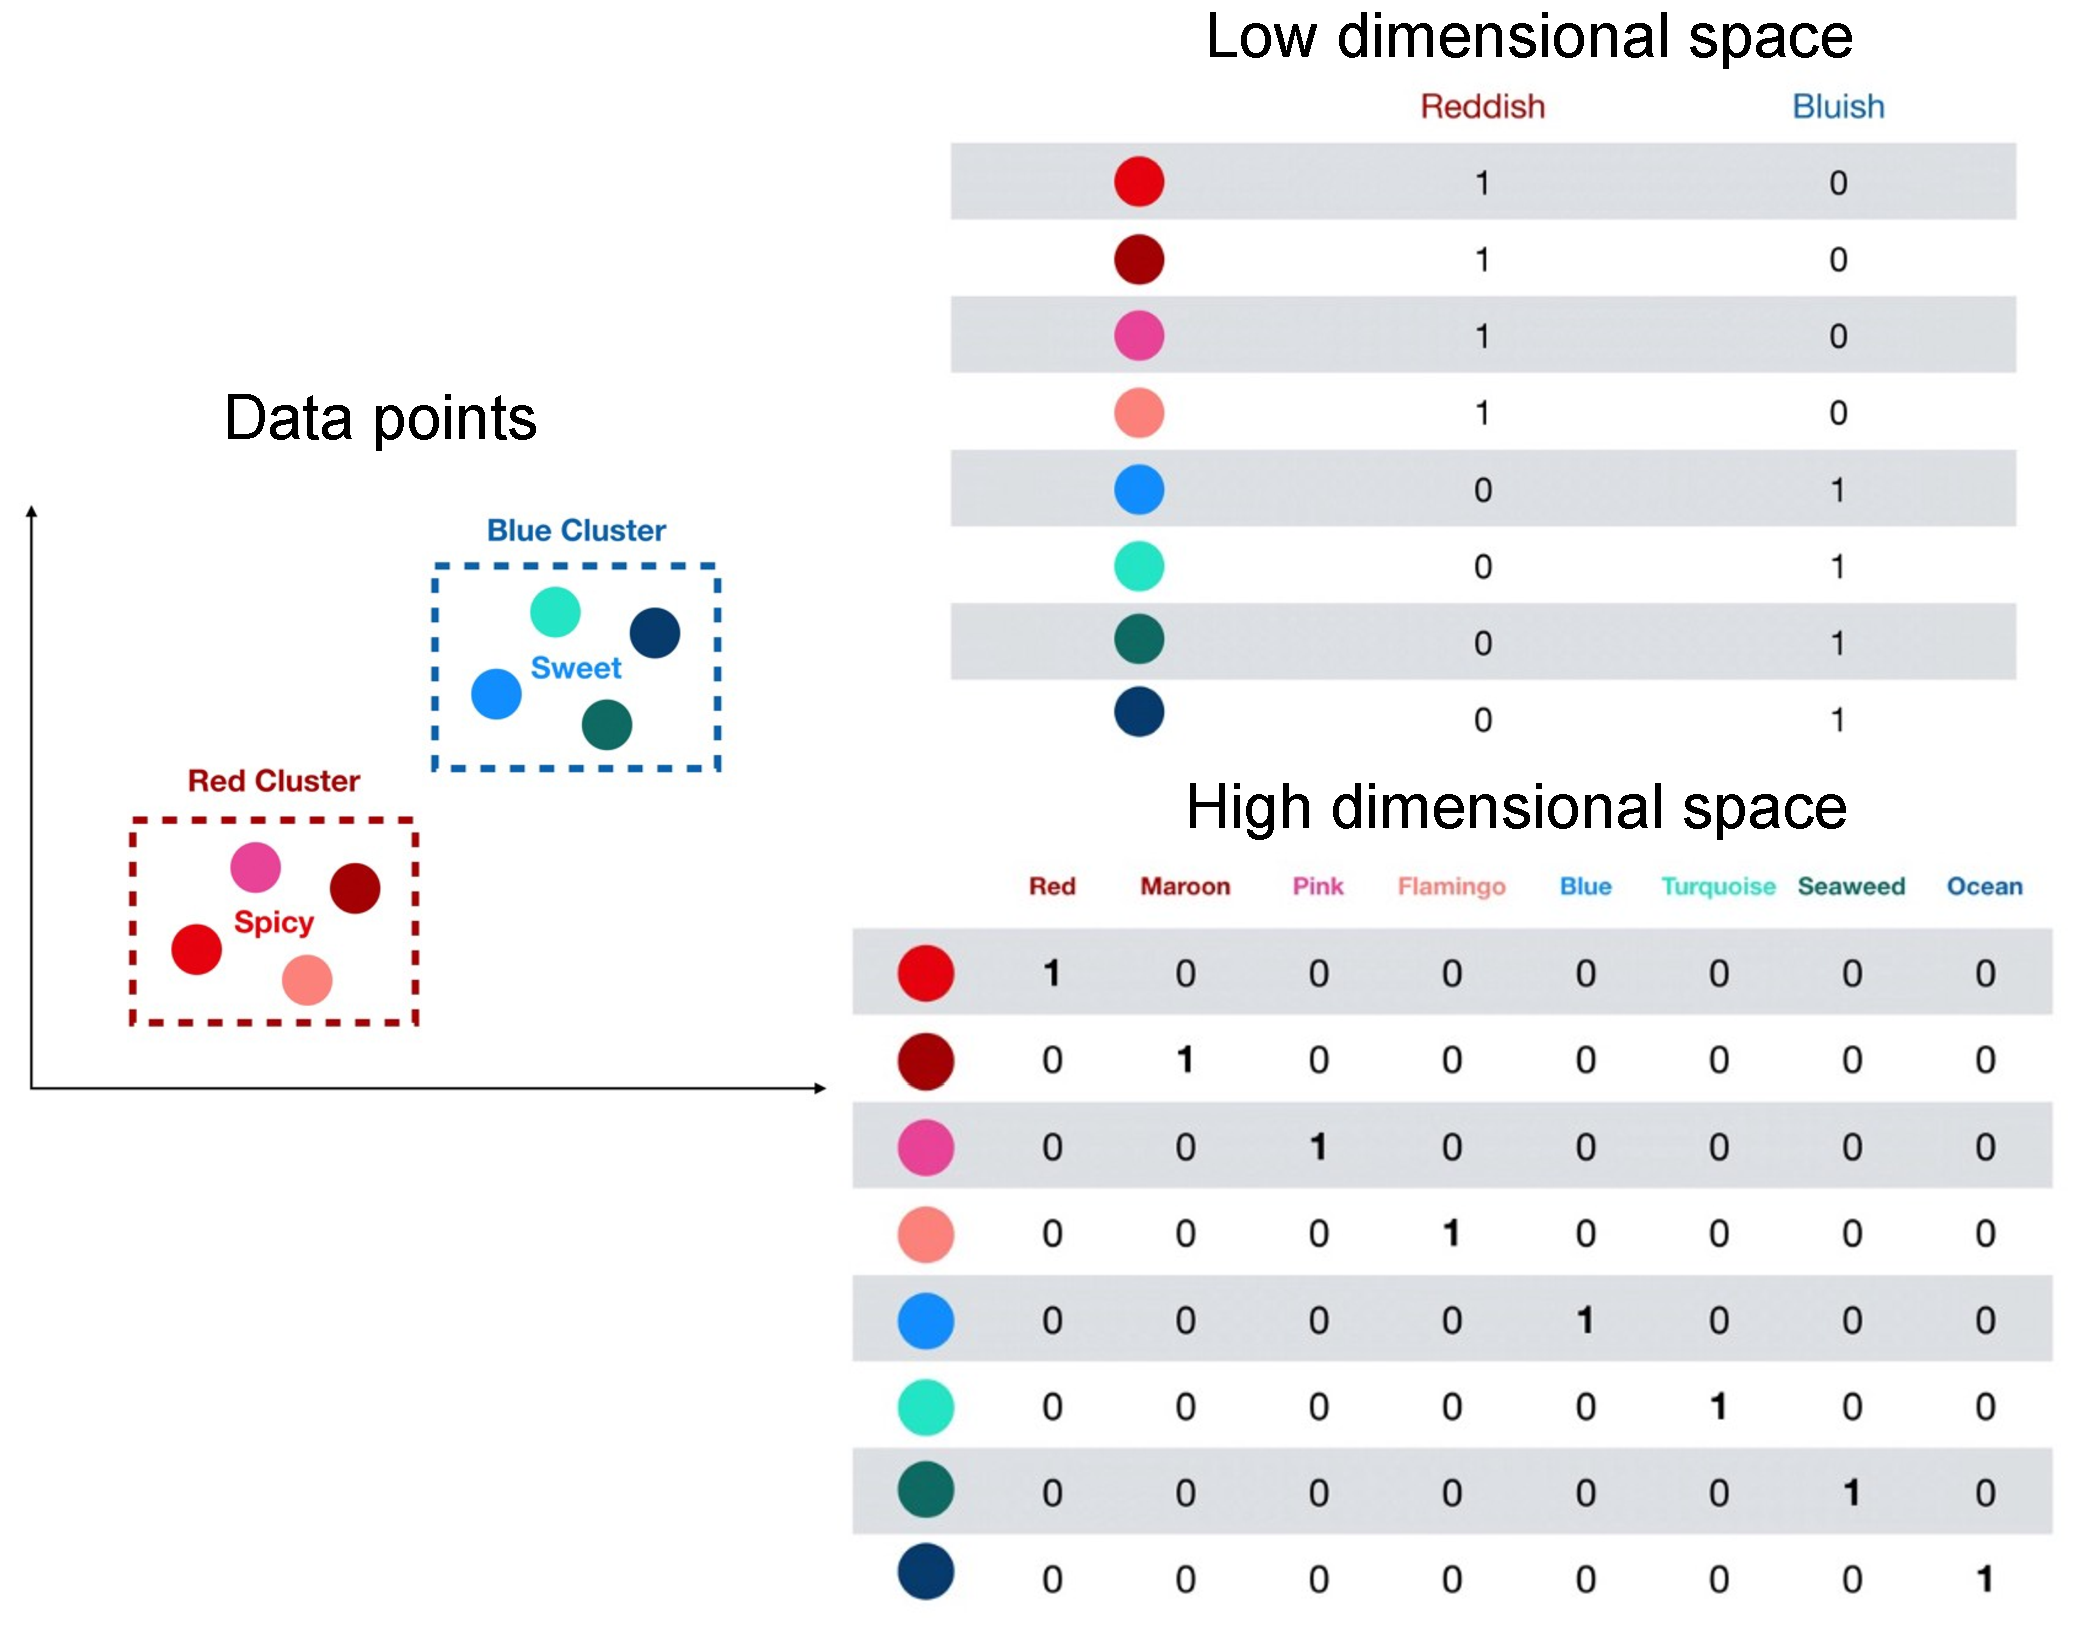
\includegraphics[width=0.7\textheight]{Images/DimRed.pdf}
\end{center}
Having a high dimensional feature space causes Euclidian distances between points to be fairly similar as the distance vector components are partitioned across many dimensions. 

%\cite{yiu}
%%Archit's comments: How exactly do we cite so that the citation appears on the slide? 

\end{frame}

\subsection{Results}

\section{Neural Network Based Approaches}

\subsection{Architectures: Feed Forward \& Recurrent Networks}


\subsection{Loss Functions: Cross Entropy vs BPMLL}

\subsection{Results}

\begin{frame}[t]
\frametitle{Artificial Neural Network Results: Full Dataset}
\begin{center}

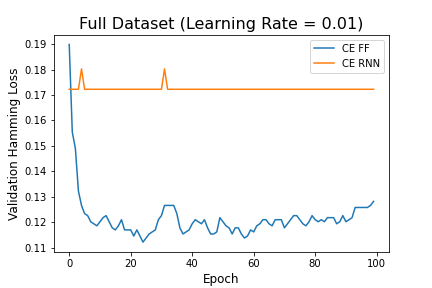
\includegraphics[width=0.32\textwidth,height=3cm]{Images/Full_Dataset_Learning_Rate_01.png}
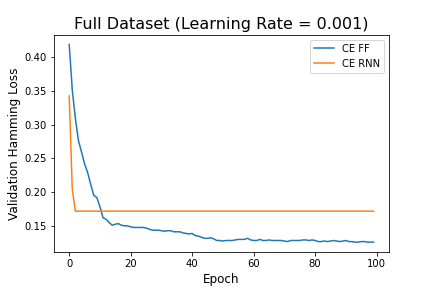
\includegraphics[width=0.32\textwidth,height=3cm]{Images/Full_Dataset_Learning_Rate_001.png}
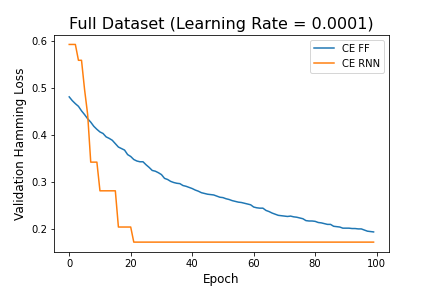
\includegraphics[width=0.32\textwidth,height=3cm]{Images/Full_Dataset_Learning_Rate_0001.png}        
\end{center}

\begin{center}

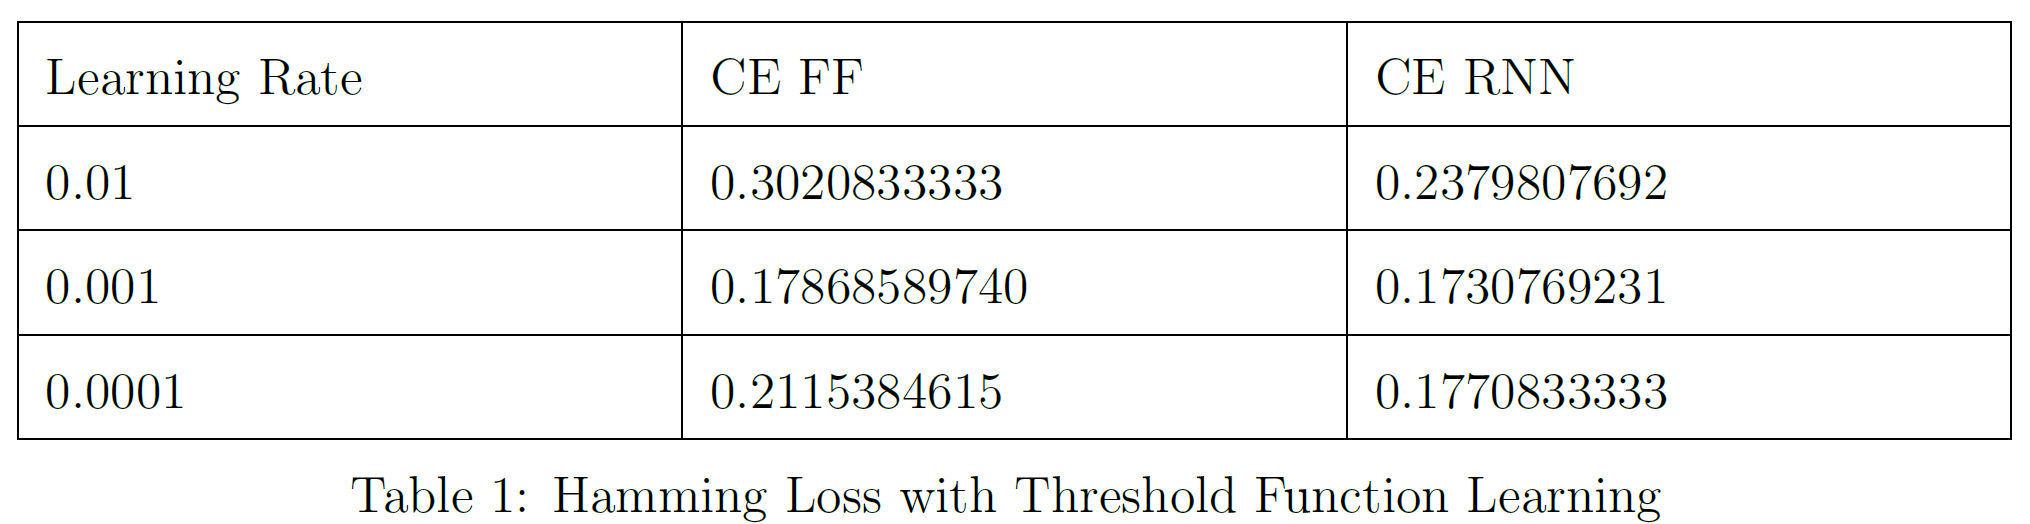
\includegraphics[width=1\textwidth,height=3cm]{Images/Threshold learning for full dataset.png}
\end{center}

CE FF outperform CE RNN in constant threshold but underperform in learned threshold; The effect of learning rate. 
\end{frame}

\begin{frame}[t]
\frametitle{Artificial Neural Network Results: Reduced Dataset}
\begin{center}

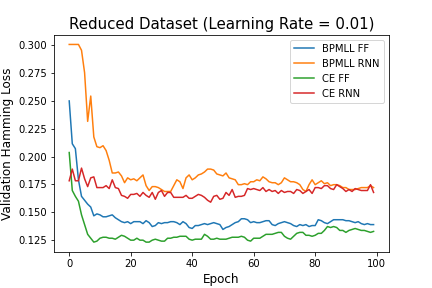
\includegraphics[width=0.32\textwidth,height=3cm]{Images/Reduced_Dataset_Learning_Rate_01.png}
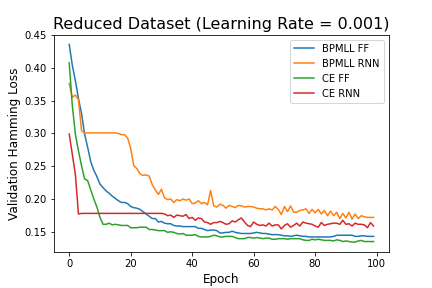
\includegraphics[width=0.32\textwidth,height=3cm]{Images/Reduced_Dataset_Learning_Rate_001.png}
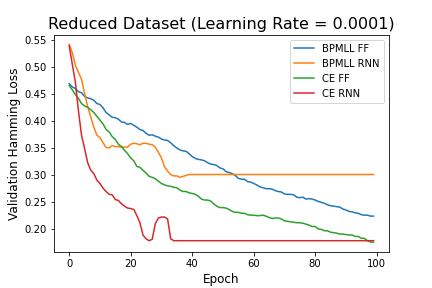
\includegraphics[width=0.32\textwidth,height=3cm]{Images/Reduced_Dataset_Learning_Rate_0001.png}        
\end{center}

\begin{center}

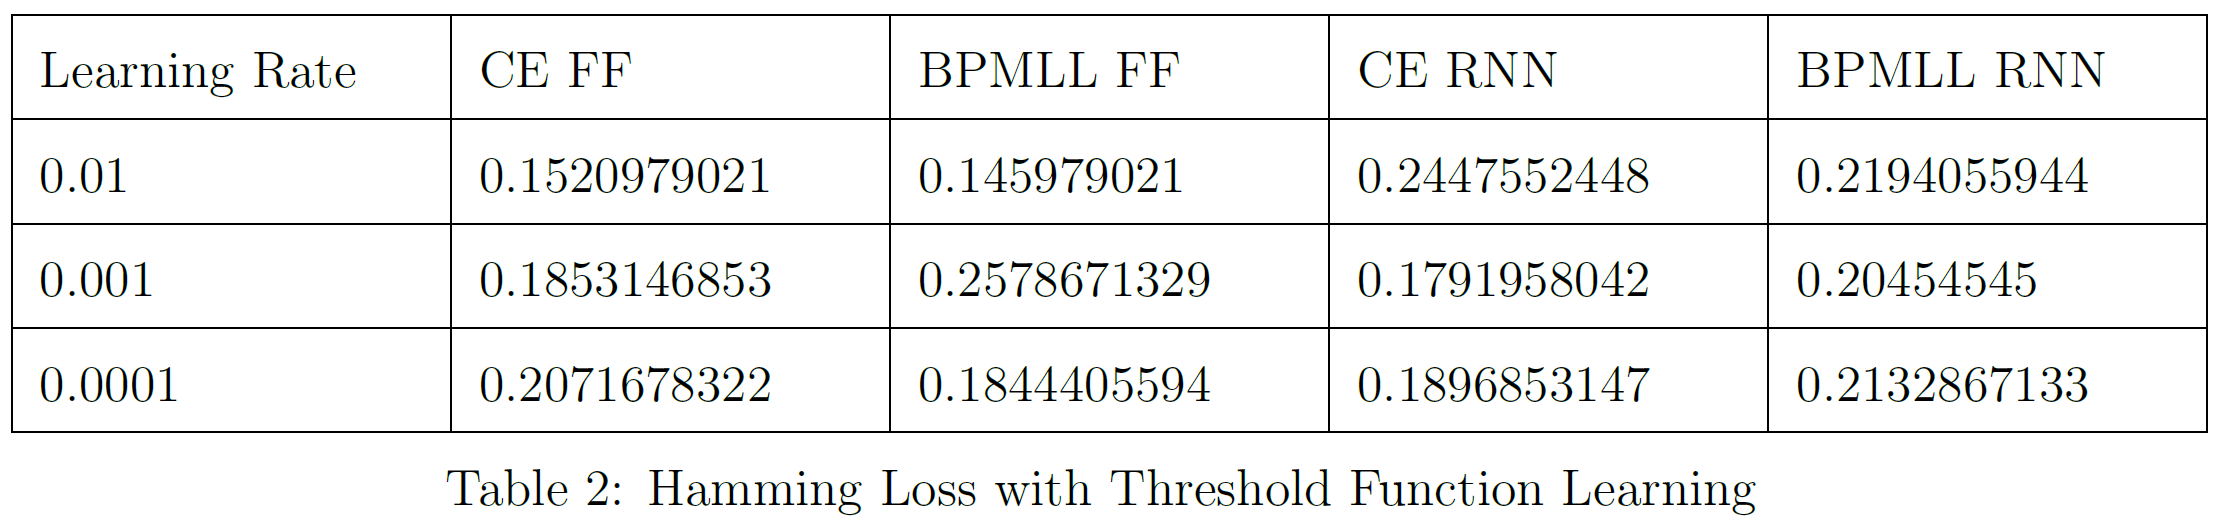
\includegraphics[width=1\textwidth,height=3cm]{Images/Threshold learning for reduced dataset.png}
\end{center}

Same conclusion for RNN and FF; BPMLL shows NO
better performance in hamming loss than cross entropy.
\end{frame}

\section{Discussion and Conclusions}

\begin{frame}[t]{References}
    \nocite{mlknn}
    \nocite{bpmll}
    \bibliography{mll_osu}
\end{frame}

\end{document}

